\documentclass[10pt,twoside]{book}
\usepackage{graphicx}
\usepackage{tcolorbox}
\usepackage{xcolor}
\usepackage{enumerate}
\usepackage{amsmath,amsthm,amssymb}
\usepackage{tabularray}
\usepackage{titlesec}
\titleformat{\chapter}{\Huge\bfseries}{\chaptername\ \thechapter}{0pt}{\vskip 20pt\raggedright}
\titlespacing{\chapter}{0pt}{-40pt}{80pt}
\UseTblrLibrary{diagbox}
\usepackage[left=2cm,right=8cm,top=2cm,bottom=1cm,marginparwidth=6cm,marginparsep=15pt]{geometry}
\usepackage{marginnote}
\usepackage{fancyhdr}
\usepackage{tikz}
\usepackage{hyperref}
\newcommand{\Font}[1]{\fontfamily{qhv}\selectfont #1}
\newtheorem*{claim}{Claim}
\newtheorem*{theorem}{Theorem}
\renewcommand{\footrulewidth}{0pt}
\renewcommand\footnoterule{}
\fancypagestyle{myheader}{
	\fancyhf{}
	\fancyhead[OL,ER]{\textit{Pigeon-hole and double counting}}
	\fancyhead[OR,EL]{\thepage}
	\fancyfoot[C]{}
	\fancyheadoffset[RE,LO]{0.05cm}
	\fancyheadoffset[LE,RO]{6.5cm}
}
\fancypagestyle{firstheader}{
	\fancyhf{}
	\fancyhead[OL,OR,EL,ER]{}
	\fancyfoot[C]{}
	\let\oldheadrule\headrule
	\renewcommand{\headrule}{\color{lightgray}\oldheadrule}
	\renewcommand{\headrulewidth}{12pt}
	\fancyfoot[L]{}
}
\renewcommand\footnotetext[1]{
	\begingroup
	\renewcommand\thefootnote{}\footnote{#1}
	\addtocounter{footnote}{-1}
	\endgroup
}
\pagestyle{myheader}
\hypersetup{colorlinks=true,linkcolor=black,urlcolor=blue}
\tcbset{colback=gray!15!white,colframe=gray!75!white,arc=0pt,outer arc=0pt,bottomrule=0pt,toprule=0pt,rightrule=0pt}
\begin{document}
	\chapter*{\Font{\LARGE{Pigeon-hole and double counting}}}
	\marginnote{
		\raggedleft{\Font{\LARGE{\textbf{Chapter 1}}}}
		\begin{flushright}
				
				\href{http://crossmark.crossref.org/dialog/?doi=10.1007/978-3-662-57265-8_28&domain=pdf}{\includegraphics[scale=.08]{images/HW-1-btn.png}}
		\end{flushright}
	}[-3.5cm]
	\thispagestyle{firstheader}
	\footnotetext{\textcopyright Springer-Verlag GmbH Germany, part of Springer Nature 2018 M. Aigner,\\ G. M. Ziegler, Proofs from THE BOOK, \url{https://doi.org/10.1007/978-3-662-57265-8\_28}}
	Some mathematical principles, such as the two in the title of this chapter, are so obvious that you might think they would only produce equally obvious results. To convince you that “It ain’t necessarily so” we illustrate them with examples that were suggested by Paul Erd\H{o}s to be included in The Book. We will encounter instances of them also in later chapters.
		\marginnote{
			\includegraphics{images/HW1-pigeons.jpg}\\
			\textit{“The pigeon-holes from a bird’s perspective”}
		}
		\begin{tcolorbox}[leftrule=3mm]
			\textbf{Pigeon-hole principle}\\
			\textit{If n objects are placed in r boxes, where r $\le$ n, then at least one of the boxes contains more than one object.}
		\end{tcolorbox}
		\noindent Well, this is indeed obvious, there is nothing to prove. In the language of
		mappings our principle reads as follows: Let \textit{N} and \textit{R} be two finite sets
		with
		$$\mid N\mid = n > r = \mid R\mid,$$
		and let 
		$f : N \rightarrow R$ be a mapping.Then there exists some $a \in R$ with 
		
		$\mid f^{-1}(a)\mid \ \geq \ 2$.
		 We may even state a stronger inequality: There exists some $a \in R$ with
		\begin{equation}
			\mid f^{-1}(a)\mid \ \geq \ \lceil \frac{n}{r}\rceil \tag{1} \label{e1}
		\end{equation}
		In fact, otherwise we would have $\mid f^{-1}(a)\mid $\textless$ \ \frac{n}{r}$ for all $a$, and hence $n = \sum\limits_{a \in R} \mid f^{-1}(a)\mid $\textless$ r\ \frac{n}{r} = n$, which cannot be.
		\section*{\Font{1. Numbers}}
		\begin{claim}
			Consider the numbers 1, 2, 3,...,$2n$, and take any $n+1$ of them. Then there are two among these $n+1$ numbers which are relatively prime.
		\end{claim}
		\noindent This is again obvious. There must be two numbers which are only 1 apart, and hence relatively prime.\\
		But let us now turn the condition around.
		\begin{claim}
			Suppose again A $\subseteq \{1,2,...,2n\}$ with $\mid A\mid = n + 1$.Then there are always two numbers in A such that one divides the other.
		\end{claim}
		\begin{proof}[\unskip\nopunct]
			This is not so clear. As Erd\H{o}s told us, he put this question to young Lajos Pósa during dinner, and when the meal was over, Lajos had the answer. It has remained one of Erd\H{o}s’ favorite “initiation” questions to mathematics. The (affirmative) solution is provided by the pigeon-hole principle. Write every number $a \in A$ in the form $a = 2^{k}m$, where $m$ is an odd number between 1 and $2n-1$ Since there are $n+1$ numbers in $A$, but only $n$ different odd parts, there must be two numbers in $A$ with the \textit{same} odd part. Hence one is a multiple of the other.
		\end{proof}
		\marginnote{
			Both results are no longer true if one replaces \textit{n}+1 by \textit{n}: For this consider the sets \{2, 4, 6,\dots,2\textit{n}\}, respectively \{\textit{n}+1, \textit{n}+2,\dots,2\textit{n}\}.
			}[-2cm]
		\section*{\Font{2. Sequences}}
		Here is another one of Erd\H{o}s’ favorites, contained in a paper of Erd\H{o}s and
		Szekeres on Ramsey problems.
		\begin{claim}
			In any sequence $a_1,a_2,...,a_{mn+1}$ of mn + $1$ distinct real
			numbers, there exists an increasing subsequence\\
			$$a_{i_{1}}\ \textless\ a_{i_{2}}\ \textless\ \dots \textless\ a_{i_{m+1}} \qquad (i_1 < i_2 < \dots <i_{m+1})$$
			of length $m$ + $1$, or a decreasing subsequence\\
			$$a_{j_{1}}\ \textless\ a_{j_{2}}\ \textless\ \dots \textless\ a_{j_{n+1}} \qquad (j_1 < j_2 < \dots <j_{n+1})$$
			of length $n$ + $1$, or both.
		\end{claim}
		\begin{proof}[\unskip\nopunct]
			This time the application of the pigeon-hole principle is not immediate. Associate to each $a_i$ the number $t_i$ which is the length of a \textit{longest increasing} subsequence starting at $a_i$. If $t_i \geq m + 1$for some $i$, then we have an increasing subsequence of length $m +1$. Suppose then that $t_i \leq
			m$ for all $i$. The function $f : a_i \rightarrow t_i$ mapping \{$a_1,\dots , a_{mn+1}$\} to \{1,\dots,m\} tells us by (\ref{e1}) that there is some $s \in \{1,\dots,m\}$ such that $f(a_i) = s$ for $\frac{mn}{m} + 1 = n + 1$ numbers $a_i$. Let $a_{j_{1}}\ \textless\ a_{j_{2}}\ \textless\ \dots \textless\ a_{j_{n+1}} \indent (j_1 < j_2 < \dots <j_{n+1})$ be these numbers. Now look at two consecutive numbers $a_{j_i}, a_{j_{i+1}}$. if $a_{j_i} \textless a_{j_{i+1}}$, then we would obtain an increasing subsequence of length $s$ starting at $a{j_{i+1}}$, and consequently an increasing subsequence of length $s+1$starting at $a_{j_{i}}$, which cannot be since $f(a_{j_{i}}) = s$. We thus obtain a decreasing subsequence $a_{j_{1}}\ \textless\ a_{j_{2}}\ \textless\ \dots \textless\ a_{j_{n+1}}$ of length $n +1$. 
		\end{proof}
		\marginnote{
		\raggedright{
		The reader may have fun in proving that
		for mn numbers the statement remains
		no longer true in general.}
		}
		This simple-sounding result on monotone subsequences has a highly nonobvious consequence on the dimension of graphs. We don’t need here the notion of dimension for general graphs, but only for complete graphs $K_n$. It can be phrased in the following way. Let $N = \{1,\dots,n\}, n \geq 3$, and consider \textit{m} permutations $\pi_1,\dots,\pi_m$ of $N$ . We say that the permutations $\pi_i$ represent $K_n$ if to every three distinct numbers \textit{i, j, k} there exists a permutation $\pi$ in which \textit{k} comes \textit{after} both i and j. The dimension of $K_n$ is then the smallest \textit{m} for which a representation $\pi_1,\dots,\pi_m$ exists.
		As an example we have dim($K_3$) = 3 since any one of the three numbers
		must come last, as in $\pi_1$ = (1, 2, 3), $\pi_2$ = (2, 3, 1), $\pi_3$ = (3, 1, 2). What about $K_4$? Note first $dim(K_n) \leq dim(K_{n+1})$: just delete $n + 1$ in a representation of $K_{n+1}$. So, $dim(K4) \geq 3$, and, in fact, $dim(K_4) =3 $, by
		taking
		$$\pi_1 = (1, 2, 3), \pi_2 = (2, 3, 1), \pi_3 = (3, 1, 2).$$
		It is not quite so easy to prove dim($K_5$) = 4, but then, surprisingly, the
		dimension stays at 4 up to \textit{n} = 12, while dim($K_13$) = 5. So dim($K_n$) seems to be a pretty wild function. Well, it is not! with \textit{n} going to infinity, dim($K_n$) is, in fact, a very well-behaved function -- and the key for finding a lower bound is the pigeon-hole principle. We claim
		\marginnote{
			\raggedright{
			$\pi_1$: 1  2  3  5  6  7  8  9 10 11 12  4\\
			\ $\pi_2$: 2  3  4  8  7  6  5 12 11 10  9  1\\
			\ $\pi_3$: 3  4  1 11 12  9 10  6  5  8  7  2\\
			\ $\pi_4$: 4  1  2 10  9 12 11  7  8  5  6  3\\
			These four permutations represent $K_{12}$
			}
			}
		\begin{equation*}
			dim(K_n) \geq \log_{2}\log_{2}n \tag{2} \label{e2}
		\end{equation*}
		Since, as we have seen, dim($K_n$) is a monotone function in \textit{n}, it suffices to verify (\ref{e2}) for $n =2^{2^{p}} + 1$, that is, we have to show that
		$$dim(K_n) \geq p + 1\indent \text{for}\indent n =2^{2^{p}} + 1$$
		\begin{proof}[\unskip\nopunct]
			Suppose, on the contrary, $dim(K_n) \leq p$, and let $\pi_1,\dots,\pi_m$ be representing permutations of $N = {1, 2,...,2^{2^{p}} + 1}$. Now we use our result on mono-tone subsequences \textit{p} times. In $\pi_1$ there exists a monotone subsequence $A_1$ of length $2^{2^{p-1}} + 1$ (it does not matter whether increasing or decreasing). Look at this set $A_1$ in $\pi_2$. Using our result again, we find a monotone subsequence $A_2$ of $A_1$ in $\pi_2$ of length $2^{2^{p-1}} + 1$, and $A_2$ is, of course, also monotone in $\pi_1$. Continuing, we eventually find a subsequence $A_p$ of size $2^{2^{0}}+ 1 = 3$ which is monotone in \textit{all} permutations $\pi_i$. Let $A_p = (a,b,c)$,then either \textit{a\textless b\textless c} or \textit{a\textgreater b\textgreater c} in all $\pi_i$. But this cannot be, since there must be a permutation where \textit{b} comes after \textit{a} and \textit{c}.
		\end{proof}
		The right asymptotic growth was provided by Joel Spencer (upper bound) and by Füredi, Hajnal, Rödl and Trotter (lower bound):
		$$dim(K_n) = \log_{2}\log_{2}n + (\frac{1}{2} + (1))\log_{2}\log_{2}n$$
		But this is not the whole story: In 1999, Morris and Ho\c{s}ten found a method which, in principle, establishes the precise value of dim($K_n$). Using their result and a computer one can obtain the values given in the margin. This is truly astounding! Just consider how many permutations of size 1422564 there are. How does one decide whether 7 or 8 of them are required to represent $K_{1422564}$?
		\marginnote{
		dim($K_n$) $\leq 4 \Leftrightarrow n \leq$ 12\\
		dim($K_n$) $\leq 5 \Leftrightarrow n \leq$ 81\\
		dim($K_n$) $\leq 6 \Leftrightarrow n \leq$ 2646\\
		dim($K_n$) $\leq 7 \Leftrightarrow n \leq$ 1422564
		}[-1cm]
		\section*{\Font{3. Sums}}
		Paul Erd\H{o}s attributes the following nice application of the pigeon-hole principle to Andrew Vázsonyi and Marta Sved:
		\begin{claim}
			Suppose we are given \textit{n} integers $a_1,...,a_n$, which need not be distinct. Then there is always a set of consecutive numbers $a_{k+1},a_{k+2},...,a_l$ whose sum $\sum^{l}_{i=k+1}$ $a_i$ is a multiple of n.
		\end{claim}
		\begin{proof}[\unskip\nopunct]
			For the proof we set $N = {0, 1,...,n}$ and $R = {0, 1,...,n-1}$. Consider the map $f : N \rightarrow R$, where $f(m)$ is the remainder of $a_1 +\dots+a_m$ upon division by \textit{n}. Since $\mid N\mid = n + 1 \ge n = \mid R\mid$ ,it follows that there are two sums $a_1 +\dots+ a_k$, $a_1 +\dots+a_l (k \le l)$with the \textit{same} remainder, where the first sum may be the empty sum denoted by 0. It follows that
			$$\sum^{l}\limits_{i=k+1}a_i = \sum^{l}\limits_{i=1}a_i - \sum^{k}\limits_{i=1}a_i$$
			has remainder 0 -- end of proof.
		\end{proof}
		Let us turn to the second principle: counting in two ways. By this we mean the following.
		\begin{tcolorbox}[leftrule=3mm]
			\textbf{Double counting}\\
			\textit{
			Suppose that we are given two finite sets R and C and a subset $S \subseteq R \times C$. Whenever $(p, q)\in S$, then we say p and q are incident. If $r_p$ denotes the number of elements that are incident to $p \in R$ and $c_q$ denotes the number of elements that are incident to $q \in C$ then
			\begin{equation*}
				\sum\limits_{p \in R}r_p = \mid S\mid = \sum\limits_{q \in C}c_q \tag{3} \label{e3}
			\end{equation*}
			}
		\end{tcolorbox}
		Again, there is nothing to prove. The first sum classifies the pairs in \textit{S} according to the first entry, while the second classifies the same pairs according to the second entry.\\
		There is a useful way to picture the set \textit{S}. Consider the matrix $A = (a_{pq})$, the incidence matrix of \textit{S}, where the rows and columns of \textit{A} are indexed by the elements of \textit{R} and \textit{C}, respectively, with
		$$a_{pq} = \begin{cases} 
			1 & if(p,q)\in S\\
			0 & if(p,q)\notin S
		\end{cases}
		$$
		With this set-up, $r_p$ is the sum of the \textit{p}-th row of $A$ and cq is the sum of the \textit{q}-th column. Hence the first sum in (\ref{e3}) adds the entries of $A$ (that is, counts the elements in \textit{S}) by rows, and the second sum by columns.\\
		The following example should make this correspondence clear. Let $R = C = {1, 2,...,8}$, and set $S = {(i, j) :i \text{divides} j}$. We then obtain the matrix in the margin, which only displays the 1’s.
		\section*{\Font{4. Numbers again}}
				\marginnote{
			\centering
\footnotesize{
			\begin{tblr}{
		vline{2} = {2-9}{},
		hline{2} = {2-9}{},
	}
	\diagbox{R}{C} & 1 & 2 & 3 & 4 & 5 & 6 & 7 & 8 \\
	1              & 1 & 1 & 1 & 1 & 1 & 1 & 1 & 1 \\
	2              &   & 1 &   & 1 &   & 1 &   & 1 \\
	3              &   &   & 1 &   &   & 1 &   &   \\
	4              &   &   &   & 1 &   &   &   & 1 \\
	5              &   &   &   &   & 1 &   &   &   \\
	6              &   &   &   &   &   & 1 &   &   \\
	7              &   &   &   &   &   &   & 1 &   \\
	8              &   &   &   &   &   &   &   & 1 
	\end{tblr}}
		}
		Look at the table on the left. The number of 1’s in column \textit{j} is precisely the number of divisors of \textit{j}; let us denote this number by \textit{t}(\textit{j}). Let us ask how large this number \textit{t}(\textit{j}) is on the \textit{average} when \textit{j} ranges from 1 to \textit{n}. Thus, we ask for the quantity
		$$\bar{t}(n) = \frac{1}{n}\sum^{n}\limits_{j=1}t(j).$$
		How large is $\bar{t}(n)$ for arbitrary \textit{n}? At first glance, this seems hopeless. For prime numbers \textit{p} we have \textit{t}(\textit{p})=2, while for $2^k$ we obtain a large number $t(2^k) = k + 1$. So, \textit{t}(\textit{n}) is a wildly jumping function, and we surmise that the same is true for $\bar{t}(n)$. Wrong guess, the opposite is true! Counting in two ways provides an unexpected and simple answer. Consider the matrix A (as above) for the integers 1 up to n. Counting by columns we get $\sum_{j = 1}^{n}t(j)$. How many 1’s are in row \textit{i}? Easy enough, the 1’s correspond to the multiples of \textit{i}: 1\textit{i}, 2\textit{i},\dots, and the last multiple not exceeding \textit{n} is $\lfloor$$\frac{n}{i}\rfloor i$. Hence we obtain
		\marginnote{
			\begin{tabular}{l|llllllll}
				n & 1 & 2 & 3 & 4 & 5 & 6 & 7  & 8  \\ 
				\hline
				$\bar t(n)$ & 1 & $\frac{3}{2}$ & $\frac{5}{3}$ & 2 & 2 & $\frac{7}{3}$ & $\frac{16}{7}$ & $\frac{5}{2}$
			\end{tabular}
		}
		$$\bar{t}(n) = \frac{1}{n}\sum^{n}\limits_{j = 1}t(j) = \frac{1}{n}\sum^{n}\limits_{i = 1}\lfloor\frac{n}{i}\rfloor \leq \frac{1}{n}\sum^{n}\limits_{i = 1}\frac{n}{i} = \sum^{n}\limits_{i = 1}\frac{1}{i}$$
		where the error in each summand, when passing from $\lfloor\frac{n}{i}\rfloor$ to $\frac{n}{i}$ is less than 1. Now the last sum is the \textit{n}-th harmonic number $H_n$, so we obtain $H_n - 1 \le \bar{t}(n) \leq H_n$, and together with the estimates of $H_n$ on page 13 this gives
		$$
		\log{n} - 1 \le H_n - 1 - \frac{1}{n} \le \bar{t}(n) \leq H_n \le \log{n} + 1
		$$
		Thus we have proved the remarkable result that, while \textit{t}(\textit{n}) is totally erratic, the average $\bar{t}(n)$ behaves beautifully: It differs from $\log{n}$ by less than 1.
		\marginnote{
			\centering
		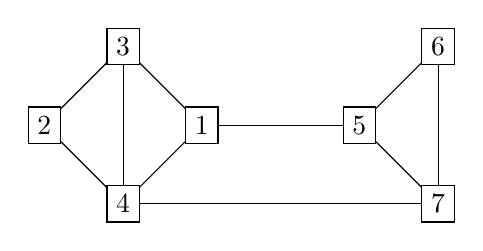
\begin{tikzpicture}
				\node[draw] (0) at (0, 0) {2};
				\node[draw] (1) at (2, 0) {1};
				\node[draw] (2) at (1, 1) {3};
				\node[draw] (3) at (1, -1) {4};
				\node[draw] (4) at (4, 0) {5};
				\node[draw] (5) at (5, 1) {6};
				\node[draw] (6) at (5, -1) {7};
				\draw (0) to (2);
				\draw (0) to (3);
				\draw (3) to (1);
				\draw (1) to (2);
				\draw (2) to (3);
				\draw (1) to (4);
				\draw (4) to (6);
				\draw (6) to (3);
				\draw (6) to (5);
				\draw (5) to (4);
		\end{tikzpicture}
		}
		\section*{\Font{5. Graphs}}
		Let \textit{G} be a finite simple graph with vertex set \textit{V} and edge set \textit{E}. We have defined in Chapter 13 the \textit{degree d}(\textit{v}) of a vertex \textit{v} as the number of edges which have \textit{v} as an end-vertex. In the example of the figure, the vertices 1, 2,\dots,7 have degrees 3, 2, 4, 3, 3, 2, 3, respectively.\\
		Almost every book in graph theory starts with the following result (that we have already encountered in Chapters 13 and 20):
		\begin{equation*}
			\sum\limits_{v \in V}d(v) = 2\mid E\mid \tag{4}\label{e4}
		\end{equation*}
		\begin{proof}[\unskip\nopunct]
			For the proof consider $S \subseteq V \times E$, where \textit{S} is the set of pairs (\textit{v}, \textit{e}) such that $v \in V$ is an end-vertex of $e \in E$. Counting \textit{S} in two ways gives on the one hand \textit{d}(\textit{v}), since every vertex contributes \textit{d}(\textit{v}) to the count, and $v \in V$ on the other hand $2\mid E\mid$, since every edge has two ends.
		\end{proof}
		As simple as the result (\ref{e4}) appears, it has many important consequences, some of which will be discussed as we go along. We want to single out in this section the following beautiful application to an extremal problem on graphs. Here is the problem:\\
		\begin{center}
	\begin{minipage}{0.8\textwidth}
	\textit{Suppose G = (V,E) has n vertices and contains no cycle of length} 4 \textit{(denoted by $C_4$), that is, no subgraph
		{\scriptsize
			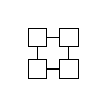
\begin{tikzpicture}
				\node[draw] (0) at (0, 0.4) {};
				\node[draw] (1) at (0.4, 0.4) {};
				\node[draw] (2) at (0.4, 0) {};
				\node[draw] (3) at (0, 0) {};
				\draw (1) to (0);
				\draw (0) to (3);
				\draw (3) to (2);
				\draw (2) to (1);
			\end{tikzpicture}
		}
		How many edges can G have at most?}
		
	\end{minipage}
			\marginnote{
				\centering
			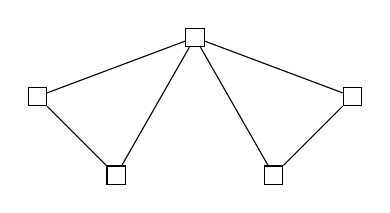
\begin{tikzpicture}
				\node[draw] (0) at (1, 0) {};
				\node[draw] (1) at (-1, 0) {};
				\node[draw] (2) at (0, 1.75) {};
				\node[draw] (3) at (2, 1) {};
				\node[draw] (4) at (-2, 1) {};
				\draw (2) to (4);
				\draw (4) to (1);
				\draw (1) to (2);
				\draw (2) to (0);
				\draw (0) to (3);
				\draw (3) to (2);
			\end{tikzpicture}
			}
		\end{center}
		As an example, the graph in the margin on 5 vertices contains no 4-cycle and has 6 edges. The reader may easily show that on 5 vertices the maximal number of edges is 6, and that this graph is indeed the only graph on 5 vertices with 6 edges that has no 4-cycle.\\
		Let us tackle the general problem. Let \textit{G} be a graph on \textit{n} vertices without a 4-cycle. As above we denote by \textit{d}(\textit{u}) the degree of \textit{u}. Now we count the following set \textit{S} in two ways: \textit{S} is the set of pairs (\textit{u},{\textit{v},\textit{w}}) where
		\textit{u} is adjacent to \textit{v} and to \textit{w}, with $v \neq w$. In other words, we count all occurrences of
		$$
		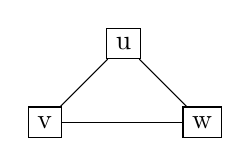
\begin{tikzpicture}
			\node[draw] (0) at (0, 1) {u};
			\node[draw] (1) at (-1, 0) {v};
			\node[draw] (2) at (1, 0) {w};
			\draw (0) to (1);
			\draw (1) to (2);
			\draw (2) to (0);
		\end{tikzpicture}
		$$
		Summing over \textit{u}, we find $\mid S \mid = \sum_{u \in V}\begin{pmatrix} d(u) \\ 2 \end{pmatrix}$ On the other hand, every pair ${v, w}$ has at most one common neighbor (by the $C_4$-condition). Hence $\mid S\mid \leq \begin{pmatrix} n \\ 2 \end{pmatrix}$ and we conclude
		$$\sum\limits_{u \in V}\begin{pmatrix} d(u) \\ 2 \end{pmatrix} \leq \begin{pmatrix} n \\ 2 \end{pmatrix}$$
		or
		\begin{equation*}
			\sum\limits_{u \in V}d(u)^{2} \leq n(n - 1) + \sum\limits_{u \in V}d(u)
			\label{e5} \tag{5}
		\end{equation*}
		Next (and this is quite typical for this sort of extremal problems) we apply the Cauchy–Schwarz inequality to the vectors $(d(u_1),...,d(u_n))$ and (1, 1,...,1), obtaining
		$$
			\left(\sum\limits_{u \in V}d(u)\right)^2 \leq n\sum\limits_{u \in V}d(u)^2
		$$
		and hence by (\ref{e5})
		$$
		\left(\sum\limits_{u \in V}d(u)\right)^2 \leq n^2(n-1) + n\sum\limits_{u \in V}d(u)
		$$
		invoking (\ref{e4}) we find
		$$
		4\mid E\mid^2 \leq n^2(n - 1) + 2n\mid E\mid
		$$
		or
		$$
		\mid E\mid^2 - \frac{n}{2}\mid E\mid - \frac{n^2(n - 1)}{4} \leq 0.
		$$
		Solving the corresponding quadratic equation we thus obtain the following result of Istvan Reiman.
		
		\begin{theorem}
			If the graph $G$ on $n$ vertices contains no 4-cycles, then
			\begin{equation}
				|E| \leq \left\lfloor \frac{n}{4} \left(1 + \sqrt{4n - 3}\right) \right\rfloor. \tag{6}
			\end{equation}
			For $n = 5$, this gives $|E| \leq 6$, and the graph above shows that equality can hold.
		\end{theorem}
		
		Counting in two ways has thus produced in an easy way an upper bound on the number of edges. But how good is the bound (6) in general? The following beautiful example [2] [3] [6] shows that it is almost sharp. As is often the case in such problems, finite geometry leads the way.\\
		In presenting the example we assume that the reader is familiar with the finite field $\mathbb{Z}_p$ of integers modulo a prime p (see page 20) 
		Consider the 3-dimensional vector space $X$ over $\mathbb{Z}_p$ We construct from $X$ the following graph $G_p$. The vertices of $G_p$ are the one-dimensional subspaces $[v] := \text{span}_{\mathbb{Z}_p}\{v\},\ 0 \neq v \in X$ , and we connect two such subspaces $[v] \neq [w]$ by an edge if
		$$\langle v, w \rangle = v_1w_1 + v_2w_2 + v_3w_3 = 0$$
		\marginnote{
			\includegraphics[scale=.3]{images/G1.png}\\
			The graph $G_2$: its vertices are all seven nonzero triples (\textit{x,y,z}).
		}
		Note that it does not matter which vector$\neq{0}$ we take from the subspace. In the language of geometry, the vertices are the points of the projective plane over $\mathbb{Z}_p$, and [w] is adjacent to [v] if w lies on the polar line of v.\\
		As an example, the graph G2 has no 4-cycle and contains 9 edges, which almost reaches the bound 10 given by (6). We want to show that this is true for any prime p.\\
		Let us first prove that Gp satisfies the $C_4$-condition. If [u] is a common neighbor of $[v]$ and $[w]$, then u is a solution of the linear equations
		\begin{equation*}
			\begin{aligned}
				v_1x + v_2y + v_3z &= 0 \\
				w_1x + w_2y + w_3z &= 0
			\end{aligned}
		\end{equation*}
		Since v and w are linearly independent, we infer that the solution space has dimension 1, and hence that the common neighbor [u] is unique Next, we ask how many vertices $G_p$ has. It’s double counting again. The space $X$ contains $p^3-1$ vectors $\neq{0}.$ Since every one-dimensional sub-space contains $p-1$ vectors $\neq{0}$ , we infer that $X$ has $\frac{p^3 - 1}{p - 1} = p^2 + p + 1$ one-dimensional subspaces, that is , $G_p$ has $n = p^2 + p + 1 $ vertices. similarly, any two-dimensional subspace contains $p^2-1$ vectors$\neq{0}$ , and hence $\frac{p^2-1}{p-1} = p+1$  one-dimensional subspaces.\\
		It remains to determine the number of edges in $G_p$, or, what is the same by (4), the degrees. By the construction of $G_p$, the vertices adjacent to $[u]$ are the solutions of the equation 
		$$u_1x +  u_2y + u_3z = 0.$$
		The solution space of (7) is a two-dimensional subspace, and hence there are $p + 1$ vertices adjacent to $[u]$. But beware, it may happen that $u$ itself is a solution of (7). In this case there are only p vertices adjacent to $[u]$.\\
		In summary, we obtain the following result: If $u$ lies on the conic given by $x^2 + y^2 + z^2 = 0$, then $d([u]) = p$, and, if not, then$ d([u]) = p + 1$. So it remains to find the number of one-dimensional subspaces on the conic $$x^2 + y^2 + z^2 = 0$$
		Let us anticipate the result which we shall prove in a moment
		\begin{claim}
			There are precisely $p^2$ solutions $(x, y, z)$ of the equation $x^2 + y^2 + z^2 = 0$, and hence (excepting the zero solution) precisely $\frac{p^2-1}{p-1} = p+1$ vertics in $G_p$ of degree $p$.
		\end{claim}
		\noindent With this, we complete our analysis of $G_p$. There are $p + 1$ vertices of degree $p$, hence $(p^2 + p + 1) - (p + 1) = p^2$ vertices of degree $p + 1$. Using $(4)$, we obtain
		\begin{align*}
			|E| &= \frac{(p+1)p}{2} + \frac{p^2(p+1)}{2} = \frac{(p+1)^2 p}{2} \\  &=  \frac{(p+1)p}{4}(1+(2p+1)) = \frac{p^2 + p}{4}(1+\sqrt{4p^2 + 4p + 1})
		\end{align*}
		
		Setting $n = p^2 + p + 1$, the last equation reads
		$$|E| = \frac{n-1}{4}(1+\sqrt{4n-3})$$
		and we see that this almost agrees with (6).\\
		Now to the proof of the claim. The following argument is a beautiful application of linear algebra involving symmetric matrices and their eigenvalues.We will encounter the same method in Chapter 44, which is no coincidence: both proofs are from the same paper by Erdos, Rényi and Sós. ˝We represent the one-dimensional subspaces of $X$ as before by vectors$v_1 , v_2 , . . . , v_p^2+p+1$, any two of which are linearly independent. Similarly, we may represent the two-dimensional subspaces by the same set of vectors, We may represent the two-dimensional subspaces by the same set of vectors, where the subspace corresponding to $u = (u_1, u_2, u_3)$ is the set of sol-utions of the equation $u_1x + u_2y + u_3z = 0$ as in (7). (Of course, this is just the duality principle of linear algebra.) Hence, by (7), a one-dimensional subspace, represented by $v_i$, is contained in the two-dimensional subspace.
		represented by vj, if and only if $<v_i , v_j > = 0.$
		Consider now the matrix A = $(a_{ij})$ of size $(p^2+p+1)\times(p^2+p+1)$, defined as follows: The rows and columns of A correspond to $v_1, \ldots, v_{p^2+p+1}$. (we use the same numbering for rows and columns) with\\
		\[
		a_{ij} = \begin{cases}
			1 & \text{if } v_i, v_j = 0 \\
			0 & \text{otherwise}
		\end{cases}
		\]
		\marginnote{
			A = $\left(\begin{array}{ccccccc}
			0 & 1 & 1 & 1 & 0 & 0 & 0 \\
			1 & 0 & 1 & 0 & 1 & 0 & 0 \\
			1 & 1 & 0 & 0 & 0 & 1 & 0 \\
			1 & 0 & 0 & 1 & 0 & 0 & 1 \\
			0 & 1 & 0 & 0 & 1 & 0 & 1 \\
			0 & 0 & 1 & 0 & 0 & 1 & 1 \\
			0 & 0 & 0 & 1 & 1 & 1 & 0 \\
		\end{array}\right)$\\
		The matrix for $G_2$
	}
		A is thus a real symmetric matrix, and we have $a_{ii}=1$ if $<v_i , v_j> = 0$ , that is precisely when $v_i$ lies on the conic $x^2 + y^2 + z^2 = 0.$ Thus all that   remains to show is that \begin{center}
			trace A = $p+1$
		\end{center}
		From linear algebra we know that the trace equals the sum of the eigenvalues. And here comes the trick: While A looks complicated, the matrix $A^2$ is easy to analyze. We note two facts:\\
		\begin{itemize}
			\item{
			Any row of $A$ contains precisely $p+1$ 1's. This implies that $p+1$ is an  eigenvalue of $A$, since $A\mathbf{1} = (p+1)\mathbf{1}$, where $\mathbf{1}$ is the vector consisting  of 1's.}
			\item{
			 For any two distinct rows vi, vj there is exactly one column with a 1 in both rows (the column corresponding to the unique subspace spanned by $v_i, v_j$)}
		\end{itemize}
		Using this fact we find\\
		\[
		A^2 = \left(\begin{array}{cccc}
			p + 1 & 1 & \dots & 1 \\
			1 & p + 1 \\
			\vdots & & \ddots \\
			& & & p + 1 \\
		\end{array}\right)
		= pI + J
		\]
		Where $I$ is the identity matrix and $J$ is the all-ones matrix. Now, $J$ has the eigenvalue $p^2 + p + 1$ (of multiplicity 1) and 0 (of multiplicity $p^2 + p$). Hence $A^2$ has the eigenvalues $p^2+2p+1 = (p+1)^2$ of multiplicity 1 and $p$ of multiplicity $p^2+p$. Since $A$ is real and symmetric, hence diagonalizable, we find that $A$ has the eigenvalue $p + 1$ or $-(p + 1)$ and $p^2 + p$ eigenvalues\\ $\pm \sqrt{p}$. From Fact 1 above, the first eigenvalue must be $p + 1$. Suppose that $\sqrt{p}$ has multiplicity $r$, and $-\sqrt{p}$ multiplicity $s$, then.\\
		\begin{center}
			trace A = $(p+1) + r\sqrt{p} - s\sqrt{p} $
		\end{center}
		But now we are home: Since the trace is an integer, we must have $r$ = $s$, so trace A = $p + 1$ \hfill $\square$
		\section*{\Font{6. Sperner's Lemma}}
		In 1912, Luitzen Brouwer published his famous fixed point theorem:
		\begin{center}\begin{minipage}{0.8\textwidth}\textit{Every continuous function $f: B^n \rightarrow B^n$ of an $n$-dimensional ball to itself has a fixed point (a point $x \in B^n$ with $f(x) = x$).}\end{minipage}\end{center}
		For dimension 1, that is for an interval, this follows easily from the inter mediate value theorem, but for higher dimensions Brouwer’s proof needed some sophisticated machinery. It was  quite a surprise when in 1928 young Emanuel Sperner (he was 23 at the time) produced a simple combinatorial result from which both Brouwer’s fixed point theorem and the invariance of the dimension under continuous bijective maps could be deduced. And what’s more, Sperner’s ingenious lemma is matched by an equally beautiful proof — it is just double counting.\\
		We discuss Sperner’s lemma, and Brouwer’s theorem as a consequence, for the first interesting case, that of dimension \textit{n} = 2. The energetic reader should find it not too difficult to extend the proofs to higher dimensions (by induction on the dimension).\\
		\marginnote{
		\includegraphics[scale=.35]{images/G2.png}
		The tricolored triangles are shaded.
		}
		\textbf{Sperner's Lemma.}\\
		\textit{Suppose that some “big” triangle with vertices $_V1$, $V_2$, $V_3$ is triangulated (that is, decomposed into a finite number of “small” triangles that fit together edge-by-edge).\\
		Assume that the vertices in the triangulation get “colors” from the set {1, 2, 3} such that $V_i$ receives the color i (for each i), and only the colors i and j are used for vertices along the edge from $V_i$ to $V_j$ (for i $\neq$ j), while the interior vertices are colored arbitrarily with 1, 2 or 3. Then in the triangulation there must be a small “tricolored” triangle, which has all three different vertex colors.}
			\begin{itemize}
				\item[\textcolor{black}{\rule{1ex}{1ex}}] \textbf{Proof.} We will prove a stronger statement: The number of tricoloredtriangles is not only nonzero, it is always odd.  the dual graph to the triangulation, but don’t take all its edges — only those which cross an edge that has endvertices with the (different) 	colors 1 and 2. Thus we get a “partial dual which has degree 1 at all vertices that correspond to tricolored triangles, degree 2 for all triangles in which the two colors 1 and 2 appear, and degree 0 for triangles that do not have both colors 1 and 2. Thus only the tricolored triangles correspond to
				\marginnote{
					\includegraphics[scale=.35]{images/G3.png}}
					vertices of odd degree (of degree 1)  However, the vertex of the dual graph which corresponds to the outside of the triangulation has odd degree: in fact, along the big edge from $V_1$ to $V_2$, there is an odd number of changes between 1 and 2. Thus an odd number of edges of the partial dual graph crosses this big edge, while the other big edges cannot have both 1 and 2 occurring as colors Now since the number of odd-degree vertices in any finite graph is even (by equation (4)), we find that the number of small triangles with three different colors (corresponding to odd inside vertices of our dual graph) is odd With this lemma, it is easy to derive Brouwer’s theorem.
				\item[\textcolor{black}{\rule{1ex}{1ex}}] \textbf{Proof of Brouwer’s fixed point theorem (for $n = 2$).} Let $\Delta$ be the triangel in $ \mathbb{R}^3 $ with vertices $e_1 = (1,0,0,)$ , $e_2 = (0,1,0)$ and $e_3 = (0,0,1)$. It suffices to prove that every continuous map $f: \Delta \rightarrow \Delta$ has a fixed point. $\Delta$ is homeomorphic to the two-dimensional ball $B^2$.\\
				We use $\delta(T)$ to denote the maximal length of an edge in a triangulation $T$. One can easily construct an infinite sequence of triangulations $T_1, T_2, \ldots$ of $\Delta$ such that the sequence of maximal diameters $\delta(T_k)$ converges to 0. Such a sequence can be obtained by explicit construction, or inductively, for example by taking $T_{k+1}$ to be the barycentric subdivision of $T_k$.\\
				For each of these triangulations, we define a 3-coloring of their vertices $v$ by setting $\lambda(v) := \min\{i : f(v)_i < v_i\}$, that is, $\lambda(v)$ is the smallest index $i$ such that the $i$-th coordinate of $f(v)-v$ is negative.If this smallest index $i$ does not exist, then we have found a fixed point and are done: to see this, 
			\end{itemize}
			note that every $v \in \Delta$ lies in the plane $x_1 + x_2 + x_3 = 1$ , hence $\sum_{i} v_i =1 .$ so if $f(v)\neq{v}$ , then at least one of the coordinates of $f(v)- v$ must be negative (and at least one must be positive).\\
			Let us check that this coloring satisfies the assumptions of Sperner’s lemma. First, the vertex $e_i$ must receive color $i$, since the only possible negative
			component of $f(e_i)-e_i$ is the $i$-th component.Moreover, if $v$ lies on the edge opposite to $e_i$, then $v_i = 0$, so the $i$-th component of $f(v)-v$ cannot be negative, and hence $v$ does not get the color $i$.\\
			Sperner’s lemma now tells us that in each triangulation $T_k$, there is a tricolored triangle $\{v_{k:1}, v_{k:2}, v_{k:3}\}$ with $\lambda(v_{k:i}) = i$. The sequence of points $(v_{k:1})_{k\geq 1}$ need not converge, but since the simplex $\Delta$ is compact some subsequence has a limit point. After replacing the sequence of triangulations $T_k$ by the corresponding subsequence (which, for simplicity we also denote by $T_k$) we can assume that $(v_{k:1})_k$ converges to a point
			$v \in \Delta$. Now the distance of $v_{k:2}$ and $v_{k:3}$ from $v_{k:1}$ is at most the mesh length $\delta(T_k)$, which converges to 0. Thus, the sequences $(v_{k:2})$ and $(v_{k:3})$ converge to the same point $v$.\\
			But where is $f(v)$? We know that the first coordinate $f(v_{k:1})$ is smaller than that of $v_{k:1}$ for all $k$. Now, since $f$ is continuous, we can derive that the first coordinate of $f(v)$ is smaller or equal to that of $v$. The same reasoning works for the second and third coordinates. Thus, none of the coordinates of $f(v) - v$ is positive — and we have already seen that this contradicts the assumption $f(v) \neq{v}$.\\
				\section*{\Font{References}}
				\begin{enumerate}[{[}1{]}]
				 \item L. E. J. Brouwer: \textit{Über Abbildungen von Mannigfaltigkeiten}, Math. Annalen 71 (1912), 97-115.
				
				 \item W. G. Brown: \textit{On graphs that do not contain a Thomsen graph}, Canadian Math. Bull. 9 (1966), 281-285.
				
				 \item P. Erdős, A. Rényi \& V. Sós: \textit{On a problem of graph theory}, Studia Sci. Math. Hungar. 1 (1966), 215-235.
				
				 \item P. Erdős \& G. Szekeres: \textit{A combinatorial problem in geometry}, Compositio Math. (1935), 463-470.
				
				 \item S. Hoşten \& W. D. Morris: \textit{The order dimension of the complete graph}, Discrete Math. 201 (1999), 133-139.
				
				 \item I. Reiman: \textit{Über ein Problem von K. Zarankiewicz}, Acta Math. Acad. Sci. Hungar. 9 (1958), 269-273.
				
				 \item J. Spencer: \textit{Minimal scrambling sets of simple orders}, Acta Math. Acad. Sci. Hungar. 22 (1971), 349-353.
				
				 \item E. Sperner: \textit{Neuer Beweis für die Invarianz der Dimensionszahl und des Gebietes}, Abh. Math. Sem. Hamburg 6 (1928), 265-272.
				
				 \item W. T. Trotter: \textit{Combinatorics and Partially Ordered Sets: Dimension Theory}, John Hopkins University Press, Baltimore and London 1992.
			\end{enumerate}
\end{document}